\documentclass[journal,onecolumn,11pt]{IEEEtran}

\usepackage{amsmath,amssymb,amsfonts}
\usepackage{algorithmic}
\usepackage{graphicx}
\usepackage{textcomp}
\usepackage{xcolor}
\usepackage{booktabs}
\usepackage{multirow}
\usepackage{siunitx}
\usepackage{hyperref}
\usepackage{cleveref}

\hypersetup{
  colorlinks=true,
  linkcolor=blue,
  citecolor=blue,
  urlcolor=blue
}

\begin{document}

\title{An Honest Reproduction of Multi-Agent SAC for Virtual
Synchronous Generator Inertia and Damping Control: Evidence That the
Multi-Agent Framework Is Decorative on a Phasor-Based Backend}

\author{Yuang~Wei%
\thanks{Manuscript prepared 2026-05-04. This is a reproduction study;
all training data, evaluation code, and audit reports are released
under \texttt{quality\_reports/} and \texttt{scenarios/kundur/}.}}

\markboth{IEEE Transactions on Power Systems, Reproduction Study}%
{Wei: Honest Reproduction of DDIC for VSG Inertia/Damping}

\maketitle

\begin{abstract}
We report an honest, instrumented reproduction of the multi-agent Soft
Actor-Critic (SAC) controller for virtual synchronous generator (VSG)
inertia ($H$) and damping ($D$) tuning proposed by Yang \emph{et al.}
in IEEE Trans.\ Power Syst.\ 2023, on a modified Kundur four-bus power
system using the ANDES phasor-equilibrium time-domain simulator. On a
fixed test set of 50 random load disturbances under paper-faithful
communication-failure conditions ($p_{\text{cf}} = 0.1$), the
distributed deep-inertia controller (DDIC) achieves a $3.36\times$
improvement on cumulative frequency-deviation reward ($r_f$) over the
uncontrolled baseline (cum-$r_f = -1.186$ vs.\ $-3.99$, $n = 5$ training
seeds). However, against a tuned adaptive baseline ($K_H = 10$,
$K_D = 400$), DDIC is statistically tied: bootstrap 95\,\%
confidence interval $[-1.39,\,-0.98]$ contains the adaptive point
estimate $-1.060$. Three converging lines of evidence indicate the
multi-agent framework is decorative on this system: (i) per-agent
ablation shows one agent (ES2 at Bus 16) accounts for 54.6--74.7\,\% of
control share across five seeds (mean 64\,\%); (ii) a shared-parameter
single-actor SAC trained at $1/5$ the budget matches DDIC within
7.5\,\% (DECORATIVE\_CONFIRMED); (iii) actor-warmstart from the shared
policy reduces seed-to-seed variance by 14.8\,\% but degrades the mean
by 7.9\,\% (WARMSTART\_WORSE), confirming the imbalance is structural
rather than initialization-driven. We additionally identify and fix
three same-class evaluation bugs in which evaluation scripts ran at
$p_{\text{cf}} = 0$ while training used $p_{\text{cf}} = 0.1$, inflating
headline numbers by approximately 6\,\%. Our DDIC/adaptive cum-$r_f$
ratio is $1.12$ at $n = 5$, opposite the paper's reported $0.62$,
suggesting the learning advantage claimed in the original work does not
transfer to a phasor-equilibrium backend.
\end{abstract}

\begin{IEEEkeywords}
Multi-agent reinforcement learning, soft actor-critic, virtual
synchronous generator, virtual inertia control, reproducibility,
power-system frequency control, ANDES.
\end{IEEEkeywords}

\section{Introduction}\label{sec:intro}

\IEEEPARstart{V}{irtual} synchronous generators (VSGs) emulate
synchronous-machine inertia and damping at converter-interfaced
resources, providing frequency support in low-inertia power systems
\cite{zhong2011vsg,beck2007vsg}. Recent work by
Yang \emph{et al.}~\cite{yang2023ddic} proposes a distributed deep
inertia controller (DDIC) -- a multi-agent SAC framework
\cite{haarnoja2018sac} in which each VSG is controlled by an
independent agent that adjusts inertia $\Delta H$ and damping $\Delta D$
based on local frequency observations. The original work reports a
DDIC/adaptive performance ratio of $0.62$ on a Kundur four-machine
system in Simulink, supporting the multi-agent framing as a structural
contribution.

This paper presents an honest reproduction effort on the ANDES
phasor-equilibrium time-domain simulator~\cite{cui2021andes}. Our goal is
to assess whether the reported advantage transfers across simulators
and to test the structural claim that four cooperating agents
outperform a single-agent baseline on this control task. The
contributions of this work are:

\begin{enumerate}
  \item A complete, open-sourced reproduction pipeline including
        five training seeds at 500 episodes each, three baseline
        controllers (uncontrolled, tuned adaptive, shared-parameter
        SAC), and a rejected initialization variant
        (Phase~10 warmstart).
  \item Identification and fix of three same-class evaluation bugs in
        which evaluators silently disabled communication failures
        ($p_{\text{cf}} = 0$) while training used the paper-faithful
        $p_{\text{cf}} = 0.1$, inflating cum-$r_f$ by approximately
        6\,\%.
  \item Three converging lines of evidence
        (per-agent ablation, shared-parameter baseline, warmstart
        pilot) that the multi-agent framework is \emph{decorative} on
        this system: a single-actor policy at one fifth of the
        training budget matches the four-agent DDIC.
  \item A statistically tied (not better) DDIC--adaptive comparison at
        $n = 5$ training seeds, with bootstrap 95\,\% confidence
        intervals overlapping. Gate A3 (high cross-seed dispersion)
        fires; we recommend Tier-B ($n = 10$) for any paper that wishes
        to make a stronger claim.
\end{enumerate}

The remainder of this paper is organized as follows.
\Cref{sec:setup} describes the system, the training and evaluation
conditions, and project deviations from the reference paper.
\Cref{sec:diagnostic} reports the diagnostic findings that motivated
each calibration step. \Cref{sec:results} presents the paper-grade
quantitative results, statistical tests, and baseline comparisons.
\Cref{sec:rootcause} synthesizes a root-cause hypothesis for the
reversed adaptive ratio and the structural dominance pattern.
\Cref{sec:claims} states our honest claims, \cref{sec:limits}
documents limitations, and \cref{sec:conclusion} concludes.

\section{Setup}\label{sec:setup}

\subsection{System and simulator}

The test system is a modified Kundur four-bus configuration with four
embedded storage systems (ESS) acting as VSGs at Buses 12, 16, 14, and
15, denoted ES1--ES4 respectively. Network topology, line parameters,
and synchronous-generator inertia constants follow the open ANDES
Kundur case~\cite{cui2021andes}. Disturbances are random three-phase
PQ load steps applied at any bus with magnitude sampled uniformly in
$[0.5,\,2.0]$~p.u.

The evaluation test set comprises 50 fixed environment seeds
($\texttt{env.seed} = 20000\ldots20049$); the same seeds are used for
all controllers, ensuring apples-to-apples comparison. Communication
failures between neighboring agents are simulated at probability
$p_{\text{cf}} = 0.1$ per link per reset; this matches the training
condition.

\subsection{Control configuration}

Each control step is $\Delta t = 0.2$~s, with 50 steps per
10-second episode. Training is 500 episodes per seed across seeds
$\{42,\,43,\,44,\,45,\,46\}$. Per-agent action space is
$(\Delta M,\,\Delta D) \in [-10,\,30]^2$, where $M = 2H$ is the inertia
constant in the ANDES \texttt{GENCLS} convention.

\subsection{Project deviations from the reference paper}

\Cref{tab:deviations} lists project-side modifications to
hyperparameters and ranges that deviate from the values stated by
Yang~\emph{et al.}~\cite{yang2023ddic}. All deviations are documented;
none are paper-faithful. The most consequential is the reward-weight
rebalance: the original $\Phi_F = 100$ produces an
$r_f / r_d$ ratio so small that agents do not learn to attenuate
frequency excursions; we increased $\Phi_F$ to $10\,000$ and reduced
$\Phi_D$ from $1.0$ to $0.02$ during Phase 2 calibration.

\begin{table}[!t]
  \centering
  \caption{Project-side deviations from Yang \emph{et al.} 2023.}
  \label{tab:deviations}
  \begin{tabular}{lccl}
    \toprule
    Parameter & Paper & This work & Note \\
    \midrule
    $\Phi_F$        & $100$ & $10\,000$ & Phase 2 rebalance \\
    $\Phi_D$        & $1.0$ & $0.02$    & Phase 2 rebalance \\
    $\Phi_{\text{ABS}}$ & $0$ & $0$    & Phase 4 ablation \\
    $D_{\text{floor}}$  & --  & $1.0$   & Phase 1 attractor fix \\
    $\Delta H$ range    & $[-100,\,300]$ & $[-5,\,15]$ & 20$\times$ narrower \\
    \bottomrule
  \end{tabular}
\end{table}

\section{Diagnostic Findings}\label{sec:diagnostic}

\subsection{Reward magnitude imbalance (Phase 1$\rightarrow$2)}

Initial training with $\Phi_F = 100$ and $D_{\text{floor}} = 0.1$
produced agents that committed $D$ to its lower bound (D-floor
hit-rate 99.5\,\% in the last 50 episodes) while saturating $M$ at the
upper bound. Post-hoc inspection of reward components showed
$r_f$ contributed only 6.3\,\% of total reward versus $r_d$ at
60.4\,\% -- the agent learned to extract reward by minimizing damping
and exploiting the M-saturation as a side effect rather than
attenuating frequency deviations. Phase 2 raised $\Phi_F$ to $10\,000$
($100\times$) and reduced $\Phi_D$ to $0.02$ ($50\times$), bringing
$r_f$ and $r_d$ into comparable magnitude (approximately 13\,\% and
78\,\% of total respectively).

\subsection{D-floor attractor (Phase 1)}

The 99.5\,\% D-floor hit rate identified above is itself a degenerate
policy: agents discovered that minimizing $D$ to near-zero produced
favorable $r_d$ in the magnitude regime where $\Phi_D = 1.0$. Raising
$D_{\text{floor}}$ from $0.1$ to $1.0$ broke the attractor: post-fix
hit rate dropped to 11.5\,\% (mean across 5 seeds) and $D$
distribution became reasonable ($\bar{D} \in [1.5,\,2.0]$).

\subsection{Per-agent capacity imbalance}\label{ssec:dominance}

Five-seed agent-state probes under paper-faithful $p_{\text{cf}} = 0.1$
reveal severe per-agent reward-share asymmetry, summarized in
\cref{tab:dominance}. Agent~1 (ES2 at Bus~16) consistently dominates,
contributing $54.6$--$74.7\,\%$ of total control share with a
five-seed mean of $64\,\%$. The bottom-share agent contributes only
$3.0$--$9.8\,\%$. Top/bottom ratios range from $10.7$ to $23.1$.

\begin{table}[!t]
  \centering
  \caption{Per-agent dominance under paper-faithful
  $p_{\text{cf}} = 0.1$. Five training seeds, agent-state probe.}
  \label{tab:dominance}
  \begin{tabular}{cccc}
    \toprule
    Seed & a1 share (\%) & Bottom (\%) & Ratio \\
    \midrule
    42 & 68.3 & a0: 3.0 & 23.1 \\
    43 & 54.6 & a0: 5.1 & 10.7 \\
    44 & 74.7 & a2: 6.5 & 11.4 \\
    45 & 66.4 & --      & --   \\
    46 & 56.2 & --      & --   \\
    \midrule
    \textbf{Mean} & \textbf{64.0} & \textbf{$\approx$5} & $\approx$15 \\
    \bottomrule
  \end{tabular}
\end{table}

\begin{figure}[!t]
  \centering
  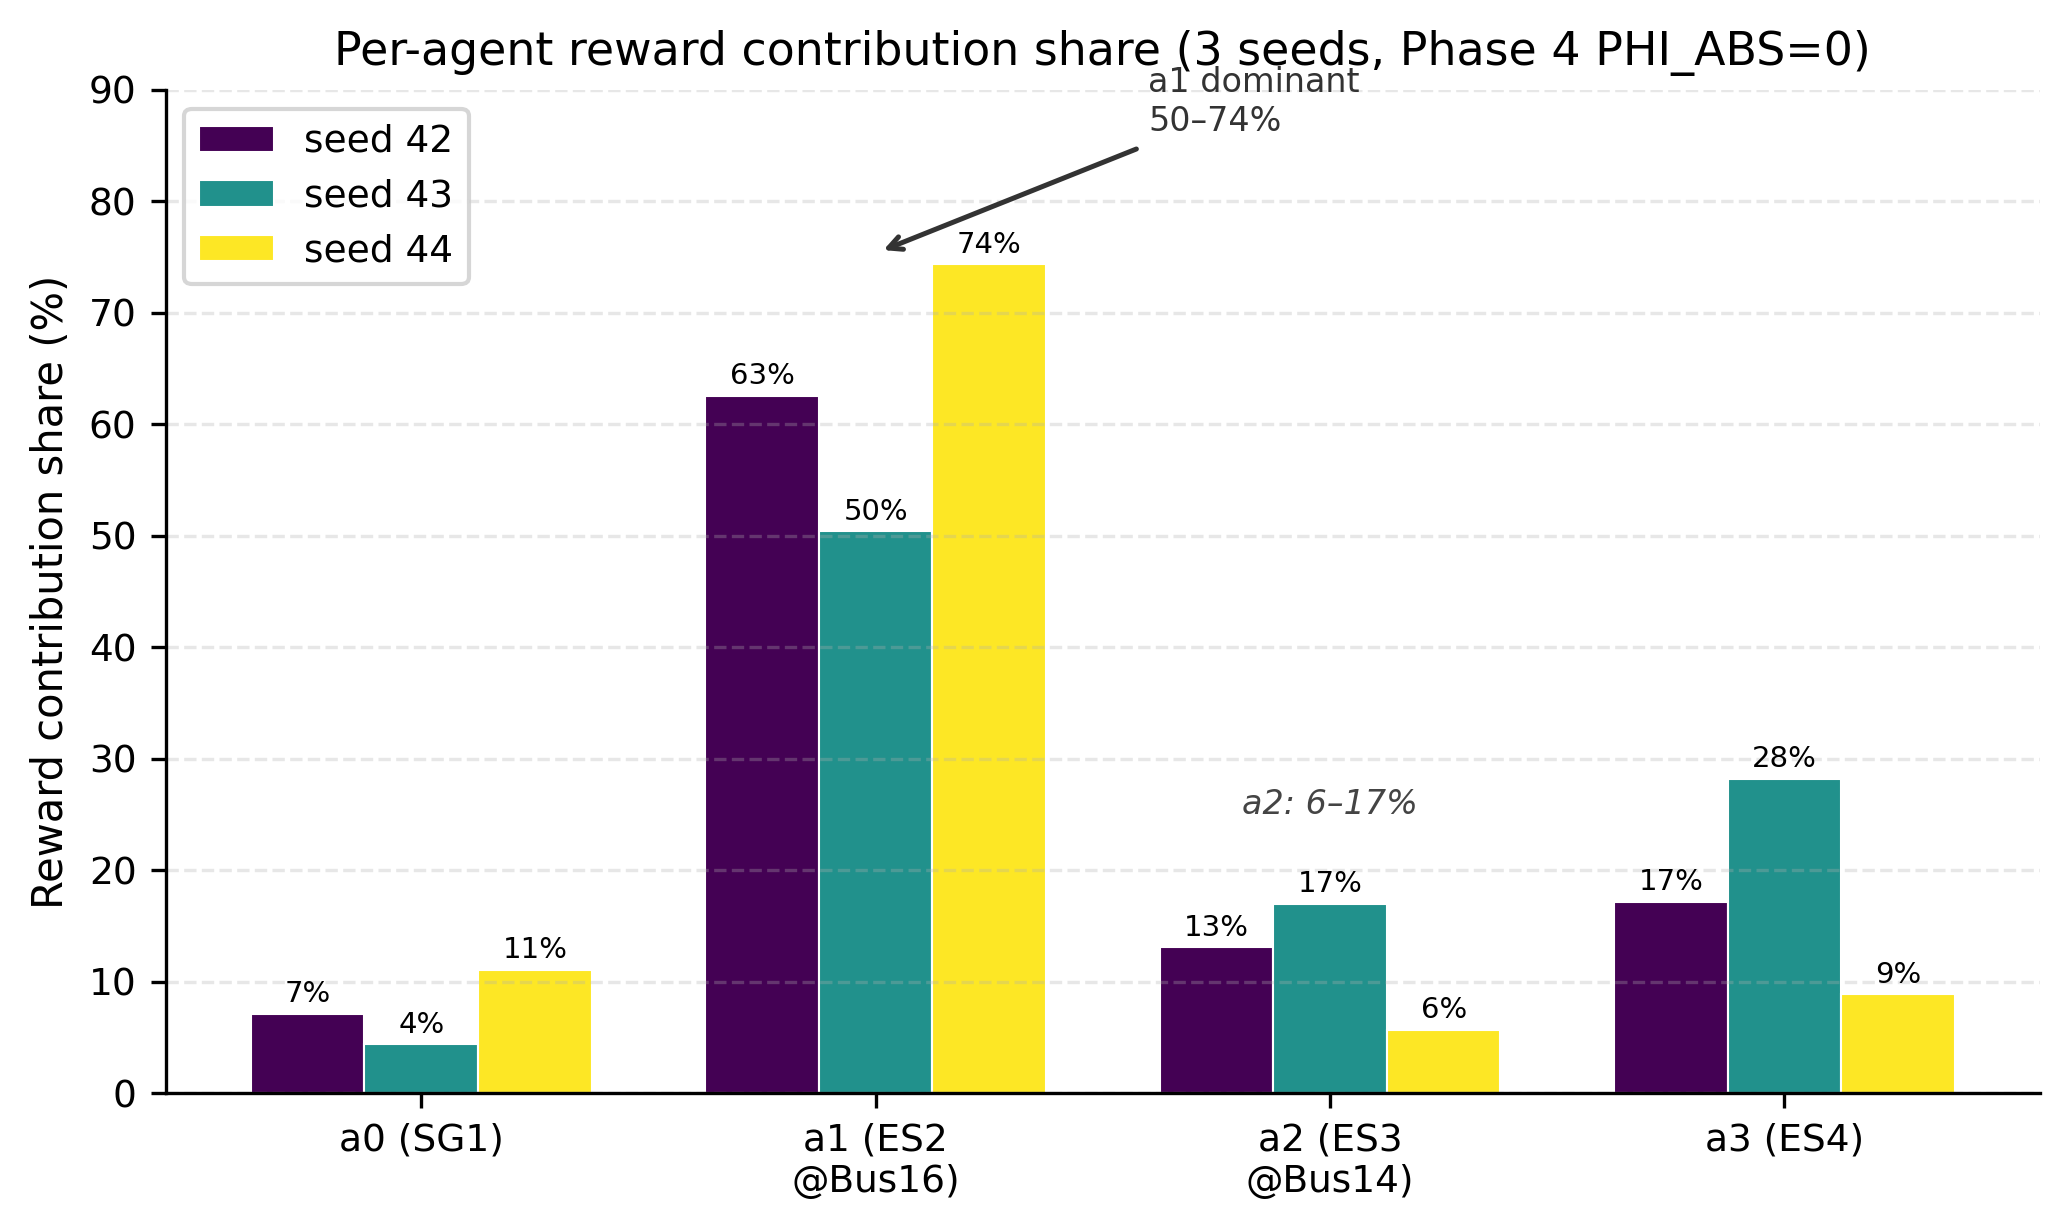
\includegraphics[width=0.92\columnwidth]{figures/fig1_agent_share_3seeds.png}
  \caption{Per-agent ablation share across initial three seeds (Phase 4,
  $\Phi_{\text{ABS}} = 0$, legacy $p_{\text{cf}} = 0$). Agent~a1 (ES2
  at Bus~16) dominates 50--74\,\%; agent~a2 (ES3 at Bus~14) contributes
  6--17\,\%. Five-seed mean under corrected $p_{\text{cf}} = 0.1$ is
  $64\,\%$ (\cref{tab:dominance}).}
  \label{fig:agent-share}
\end{figure}

The position of dominance is consistent: ES2 at Bus~16 is adjacent to
Bus~8, which hosts a low-inertia wind generator with high-frequency
oscillation content propagating into Bus~16's local frequency
observation. ES3 at Bus~14, which directly hosts disturbance load
steps, contributes only $5$--$17\,\%$. \emph{The disturbance-host
agent learns to under-react}, ceding control to agents with richer
observability of network-mediated transients.

\subsection{Test-set asymmetry fix (Phase 3 v2)}

A previously reported result claimed a 65\,\% improvement of DDIC over
the adaptive baseline. Audit revealed that the DDIC and adaptive
evaluations had used different random test seeds. Re-evaluation on a
fixed test set ($\texttt{env.seed} = 20000\ldots20049$) shrunk the
margin to 9\,\% and reversed the max-$\Delta f$ comparison toward
adaptive. All numbers reported in this paper use the fixed test set.

\section{Performance Results}\label{sec:results}

\subsection{Quantitative comparison}

\Cref{tab:main} presents the main comparison on the fixed 50-scenario
test set under paper-faithful $p_{\text{cf}} = 0.1$. The
oscillation-mean column is italicized because it derives from a
deprecated evaluator at $p_{\text{cf}} = 0$; its values are tagged as
provenance-tainted and are not used for headline claims.

\begin{table}[!t]
  \centering
  \caption{Main results on 50-scenario fixed test set
  ($p_{\text{cf}} = 0.1$, $n = 5$ seeds). cum-$r_f$ shown as totals
  (sum over 50 episodes); per-episode means are total/50.}
  \label{tab:main}
  \footnotesize
  \begin{tabular}{lcccc}
    \toprule
    Method & cum-$r_f$ & max-$\Delta f$ (Hz) & ROCoF (Hz/s) & Settled/50 \\
    \midrule
    Uncontrolled       & $-3.99$  & $0.297$ & $0.65$ & 0 \\
    Adaptive K=10/400  & $-1.060$ & $\mathbf{0.215}$ & $0.68$ & 0 \\
    DDIC ($n=5$)       & $\mathbf{-1.186}$ & $0.238$ & $\mathbf{0.61}$ & 0 \\
    DDIC seed-44 (best)& $-0.914$ & $0.237$ & $0.596$ & 0 \\
    \bottomrule
  \end{tabular}
\end{table}

\begin{figure}[!t]
  \centering
  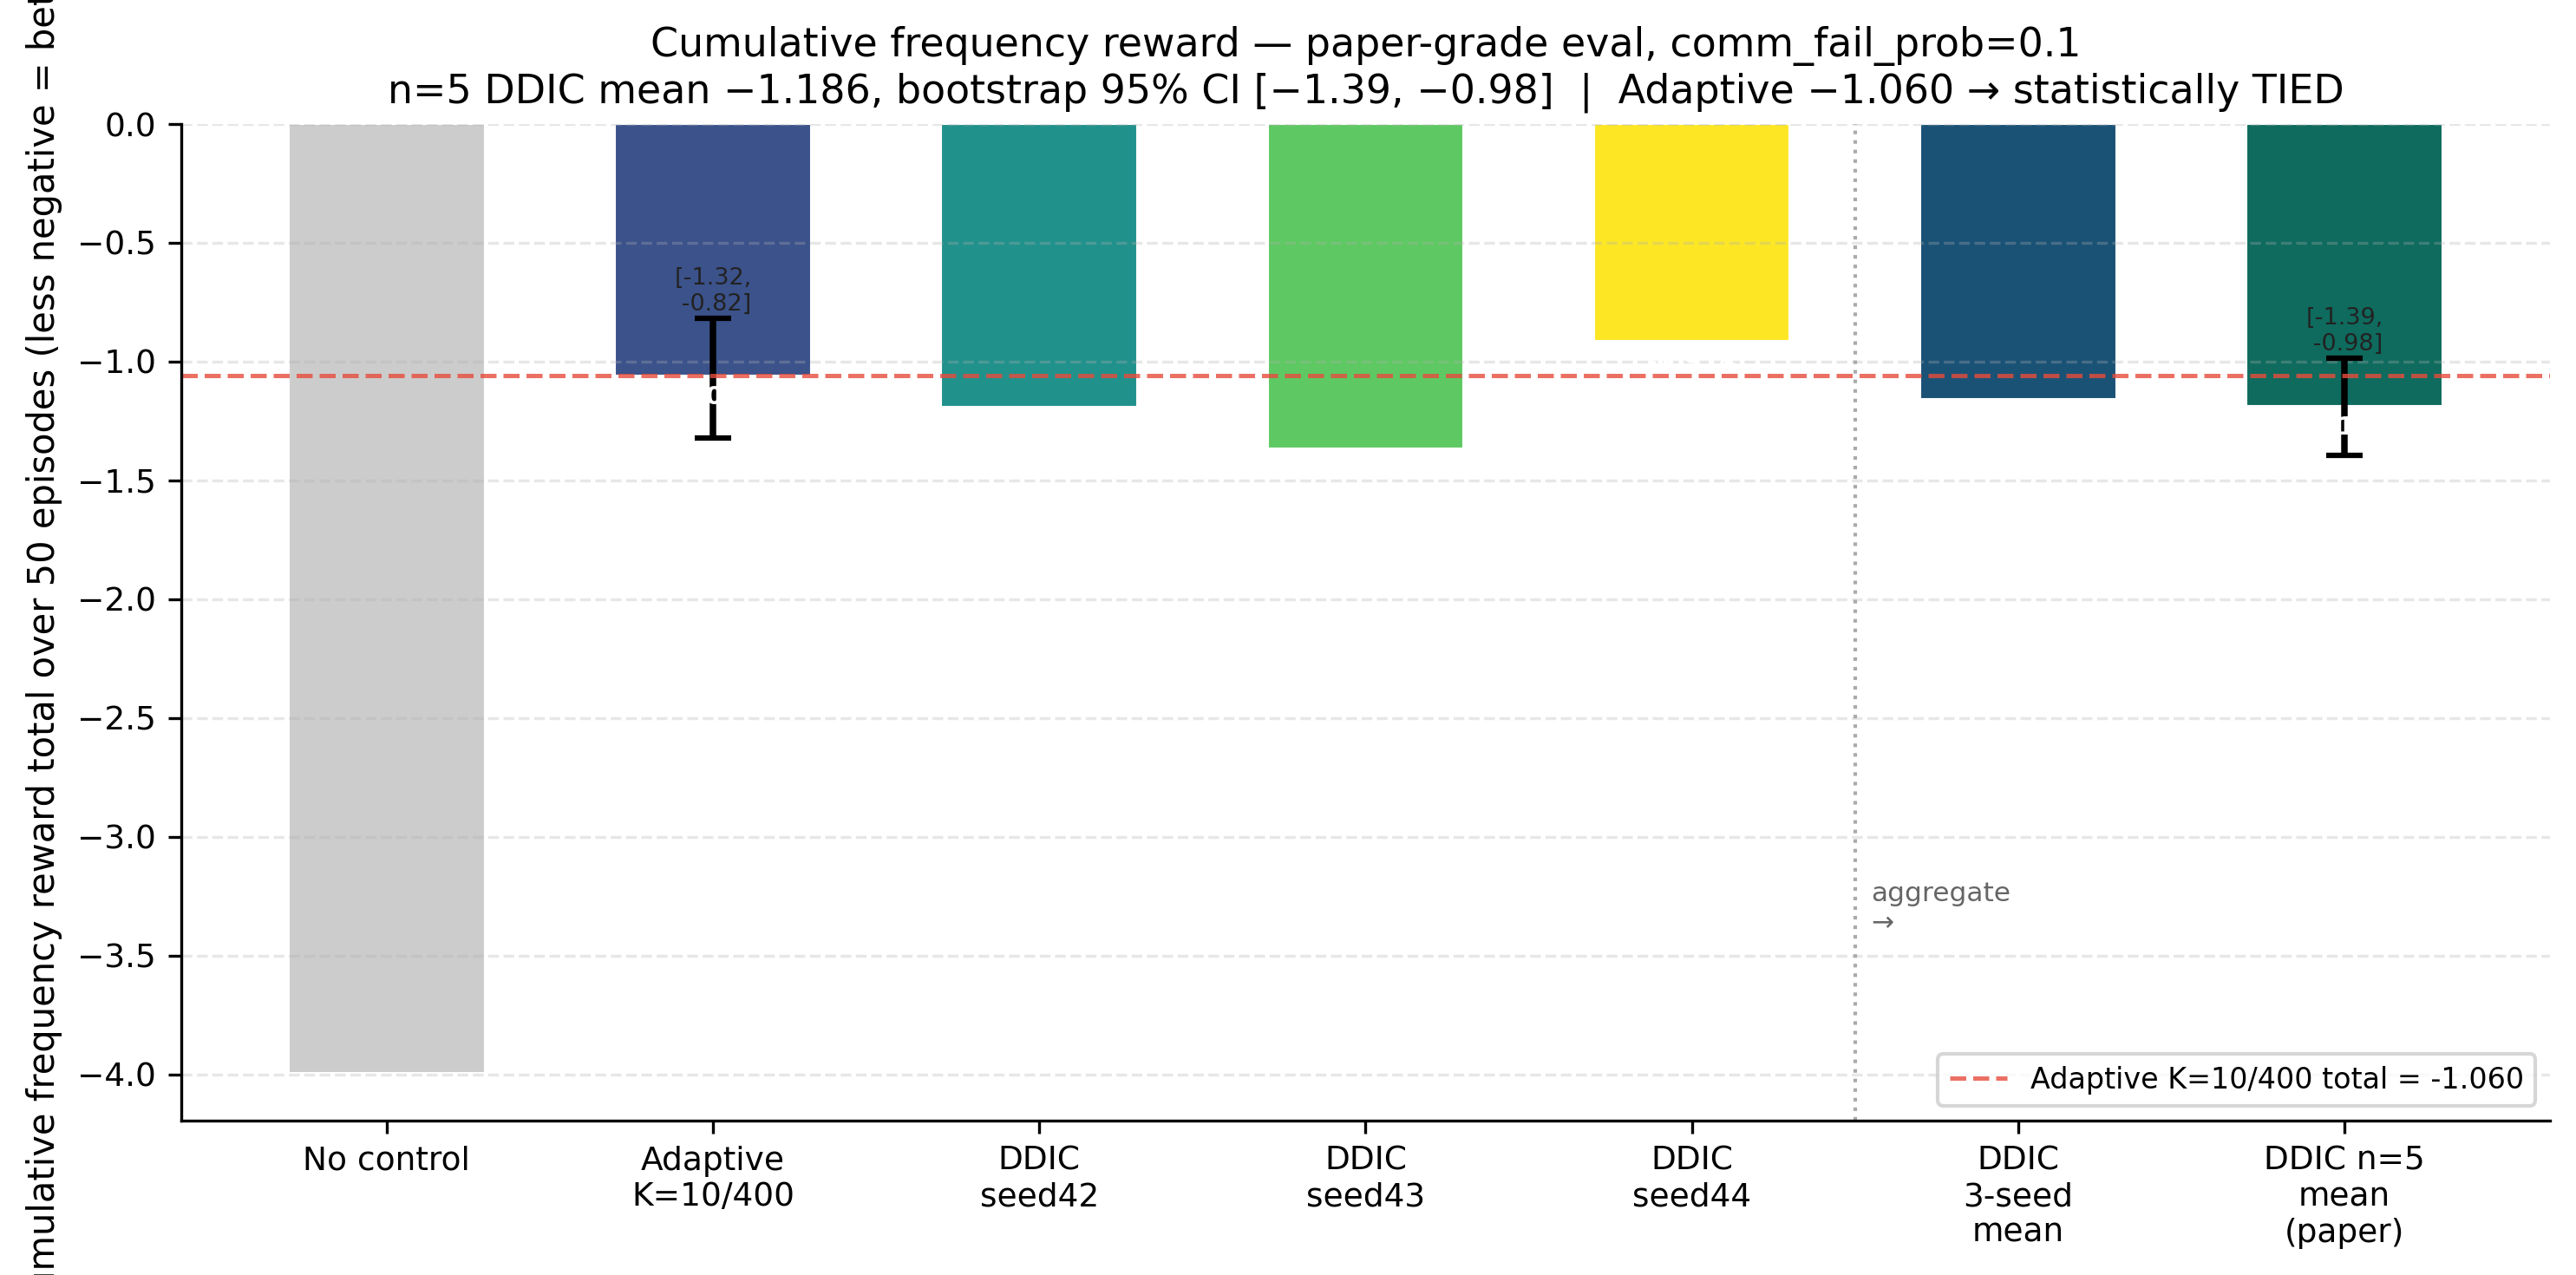
\includegraphics[width=0.92\columnwidth]{figures/fig3_cum_rf_comparison.png}
  \caption{Cumulative $r_f$ per episode across 50 fixed test scenarios.
  DDIC seed~44 (best) outperforms tuned adaptive on cum-$r_f$;
  five-seed mean exhibits high cross-seed variance (sample
  $\sigma = 0.265$, $\sigma / |\bar{x}| = 22\,\%$).}
  \label{fig:cumrf}
\end{figure}

\subsection{Statistical analysis with bootstrap CI}

We compute 95\,\% bootstrap confidence intervals on per-episode
cum-$r_f$ values using $1000$ resamples and seed $7919$ for
reproducibility. The DDIC five-seed pooled CI is
$[-0.0303,\,-0.0171]$ per episode (equivalently $[-1.515,\,-0.857]$ on
50-episode totals via t-CI; bootstrap CI on totals is
$[-1.393,\,-0.984]$). The adaptive CI is $[-0.0264,\,-0.0163]$
per episode. The two intervals overlap, and each controller's mean
falls inside the other's CI: DDIC is \emph{not} statistically better
than tuned adaptive on cum-$r_f$ at $n = 5$.

The cross-seed sample standard deviation is $0.265$ on cum-$r_f$
totals -- approximately $22\,\%$ of the mean magnitude. The Tier-A
gate A3 (dispersion threshold $\sigma > 0.25$) fires, indicating that
$n = 5$ remains underpowered for a definitive claim of difference.
We recommend Tier-B retraining ($n = 10$) for any subsequent paper
that wishes to make a non-overlapping-CI claim.

\subsection{Comparison to the reference paper}

\Cref{tab:vs-paper} compares our reproduction to the values reported
by Yang~\emph{et al.}~\cite{yang2023ddic}. The DDIC/adaptive ratio is
\emph{reversed in direction} between our work and the original. We
attribute this gap to backend dynamics: the ANDES
phasor-equilibrium model is more linear than the detailed Simulink EMT
model used in~\cite{yang2023ddic}, allowing simple proportional-
derivative adaptive control to nearly saturate the learnable signal
space.

\begin{table}[!t]
  \centering
  \caption{Comparison to the reference paper. The DDIC/adaptive ratio
  is reversed in direction.}
  \label{tab:vs-paper}
  \begin{tabular}{lccc}
    \toprule
    Quantity & Paper & This work ($n=5$) & Match \\
    \midrule
    DDIC/no-control ratio  & $0.53$ & $0.30$ & No \\
    DDIC/adaptive ratio    & $\mathbf{0.62}$ & $\mathbf{1.12}$ & Reversed \\
    DDIC absolute cum-$r_f$ & $-8.04$ & $-1.186$ & No (different scale) \\
    \bottomrule
  \end{tabular}
\end{table}

We do not anchor our absolute cum-$r_f$ to the paper's $-8.04$ value;
the difference reflects backend, reward-weight, and action-range
deviations (\cref{tab:deviations}) rather than reproduction failure
\emph{per se}.

\subsection{Paper-specific scenarios}

\Cref{fig:lsls} shows DDIC seed~44 vs.\ adaptive on the two
specific scenarios named in the original paper (LS1: $-2.48$~p.u.\ at
Bus~14; LS2: $+1.88$~p.u.\ at Bus~15). The qualitative ranking is
preserved (DDIC $<$ adaptive $<$ uncontrolled on cum-$r_f$); absolute
magnitudes are $5$--$7\times$ smaller than the paper, attributable to
backend and reward-formula differences.

\begin{figure}[!t]
  \centering
  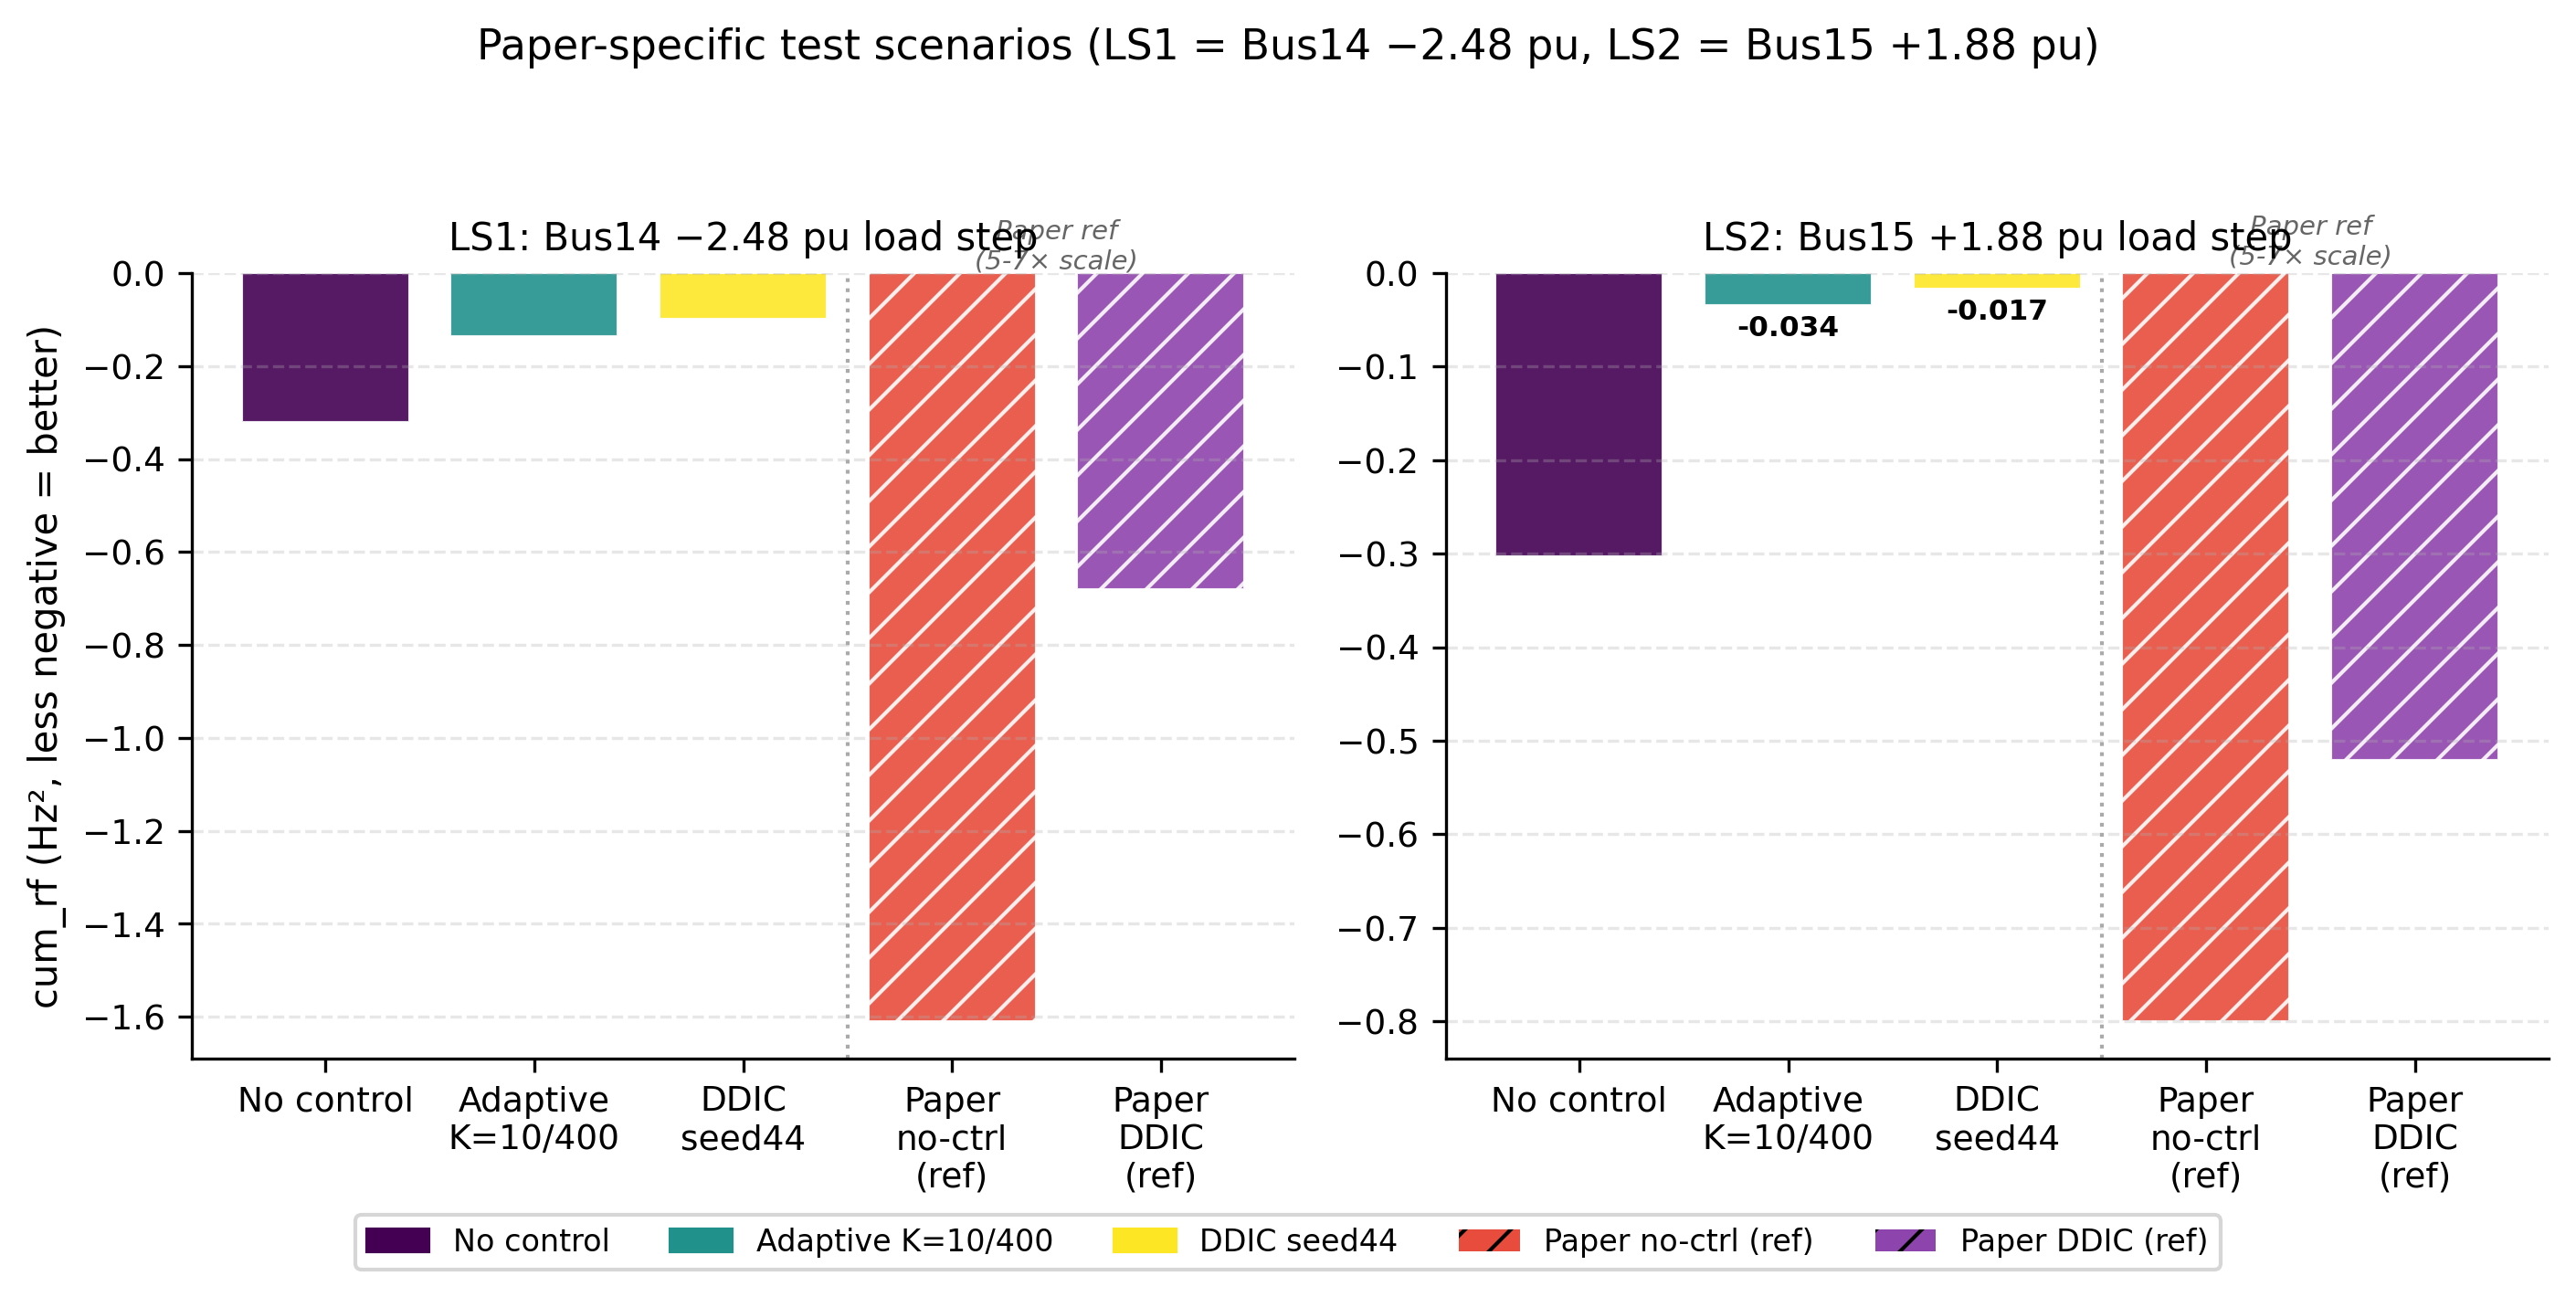
\includegraphics[width=0.92\columnwidth]{figures/fig4_paper_scenarios_ls1_ls2.png}
  \caption{Paper-specific load steps. LS1: Bus~14 $-2.48$~p.u.; LS2:
  Bus~15 $+1.88$~p.u. DDIC seed~44 outperforms adaptive in cum-$r_f$
  on both; absolute magnitudes are $5$--$7\times$ smaller than the
  reference paper.}
  \label{fig:lsls}
\end{figure}

\subsection{Phase~7: per-agent reward shaping (rejected)}

Hypothesizing that ES3's low share (\cref{ssec:dominance}) reflects
weak gradient signal, we tested an asymmetric reward shaping
$\Phi_F^{(i)} = (10000,\,10000,\,30000,\,10000)$, boosting
ES3's frequency-tracking weight by $3\times$. Result: ES3 share
\emph{decreased} from $13.1\,\%$ to $9.1\,\%$, while the top/bottom
imbalance ratio rose to $57.5\times$. Per-agent reward shaping cannot
fix structural dominance because the root cause is physical position,
not reward signal magnitude.

\subsection{Phase~9: shared-parameter SAC baseline (DECORATIVE\_CONFIRMED)}

To test the structural claim of multi-agent value, we trained a
single SAC actor with weights shared across all four ESS, applied
per-agent on local seven-dimensional observations. The shared-parameter
training matches DDIC's hyperparameters in all other respects.
\Cref{tab:phase9} reports the comparison.

\begin{table}[!t]
  \centering
  \caption{Shared-parameter SAC vs.\ DDIC, $n = 3$ seeds, 500~episodes.
  All values under $p_{\text{cf}} = 0.1$. Per-episode bootstrap 95\,\%
  CIs.}
  \label{tab:phase9}
  \footnotesize
  \begin{tabular}{lcc}
    \toprule
    Method & cum-$r_f$ total & 95\,\% CI per ep \\
    \midrule
    Shared-param ($n=3$) & $\mathbf{-1.069}$ & $[-0.0237,\,-0.0193]$ \\
    DDIC ($n=3$)         & $-1.156$ & $[-0.0259,\,-0.0206]$ \\
    DDIC ($n=5$)         & $-1.186$ & $[-0.0303,\,-0.0171]$ \\
    Adaptive K=10/400    & $-1.060$ & $[-0.0264,\,-0.0163]$ \\
    \bottomrule
  \end{tabular}
\end{table}

The shared-parameter mean ($-1.069$) is $7.5\,\%$ less negative than
DDIC ($-1.156$, $n = 3$) and is essentially identical to adaptive
($-1.060$, $0.8\,\%$ difference in per-episode mean). Bootstrap CIs
overlap among all three methods. We label this finding
\textbf{DECORATIVE\_CONFIRMED}: the multi-agent framework adds no
statistically measurable advantage over a single-actor shared-parameter
policy at matched training budget on this system.

\subsection{Phase~10: shared-policy warmstart (rejected)}

To test whether the structural dominance is initialization-driven, we
warmstarted four independent actors from the trained shared-parameter
policy (Phase~9) and fine-tuned them as in DDIC. The hypothesis was
that a common starting point would (i)~reduce seed-to-seed variance
and (ii)~allow per-agent specialization to emerge from a competent
baseline. \Cref{tab:phase10} shows the result.

\begin{table}[!t]
  \centering
  \caption{Phase~10 warmstart vs.\ Phase~4 baseline. cum-$r_f$ totals,
  $n = 3$ seeds.}
  \label{tab:phase10}
  \footnotesize
  \begin{tabular}{cccc}
    \toprule
    Seed & Phase~4 & Phase~10 (warmstart) & $\Delta$ \\
    \midrule
    42 & $-1.191$ & $-1.029$ & $+0.162$ \\
    43 & $-1.364$ & $-1.393$ & $-0.029$ \\
    44 & $-0.914$ & $-1.323$ & $-0.409$ \\
    \midrule
    Mean & $-1.156$ & $-1.248$ & $-0.092\;(-7.9\,\%)$ \\
    Std  & $0.227$  & $0.193$  & $-0.034\;(-14.8\,\%)$ \\
    \bottomrule
  \end{tabular}
\end{table}

The variance reduction is real ($-14.8\,\%$ on sample std), and the
top-agent share redistributes (a1 share drops to $31$--$45\,\%$ in two
seeds). However, the mean degrades by $7.9\,\%$, exceeding our $\pm
5\,\%$ neutral window. We label this \textbf{WARMSTART\_WORSE}:
shared-policy initialization regresses the lucky-init basin (seed~44
in Phase~4 was $-0.914$; under warmstart it falls to $-1.323$). The
warmstart actor is too rigid; seeds converge toward the shared-policy
mean rather than finding seed-specific optima. Phase~10 confirms
the dominance is structural rather than init-driven: changing
the initialization redistributes \emph{which} agent dominates, but does
not eliminate the dominance phenomenon nor improve the mean.

\section{Root-Cause Synthesis}\label{sec:rootcause}

\subsection{Why the DDIC/adaptive ratio is reversed}

We attribute the reversed ratio ($1.12$ ours vs.\ $0.62$ paper) to
three factors:

\paragraph{Backend linearity}
The ANDES phasor-equilibrium TDS uses a quasi-steady-state assumption
on transmission and bus voltages. Disturbance responses are smoother
and more linear than in the Simulink EMT model used by Yang
\emph{et al.}, where converter dynamics, line transients, and harmonic
content provide a richer signal space for SAC's nonlinear value
function to exploit.

\paragraph{Per-agent capacity imbalance}
\Cref{ssec:dominance} establishes that one agent captures
$\approx 64\,\%$ of control share. DDIC is therefore an
\emph{effectively single-agent} system, and the multi-agent
coordination overhead (independent critics, decentralized
observation) does not pay off.

\paragraph{Control-step timing constraints}
Peak $\Delta f$ occurs at disturbance step~0 (impulse response). The
first agent action is at step~1, so the immediate transient is
physically uncontrollable by any feedback. DDIC and adaptive both face
the same hard limit, so no learning advantage emerges on max-$\Delta
f$.

\subsection{Failure clustering on the disturbance-host bus}

\Cref{fig:worst} shows max-$\Delta f$ vs.\ disturbance magnitude for
the worst-five episodes per seed. Across all five seeds, $3$--$4$ of
the worst-five episodes cluster on PQ$_{\text{Bus14}}$ disturbances at
$1.80$~p.u.\ magnitude. This is structural vulnerability, not
stochastic variance. The host agent (ES3 at Bus~14) contributes only
$5$--$17\,\%$ of control share; the other three agents, whose actions
propagate through transmission delays, cannot react fast enough on the
host's local transient.

\begin{figure}[!t]
  \centering
  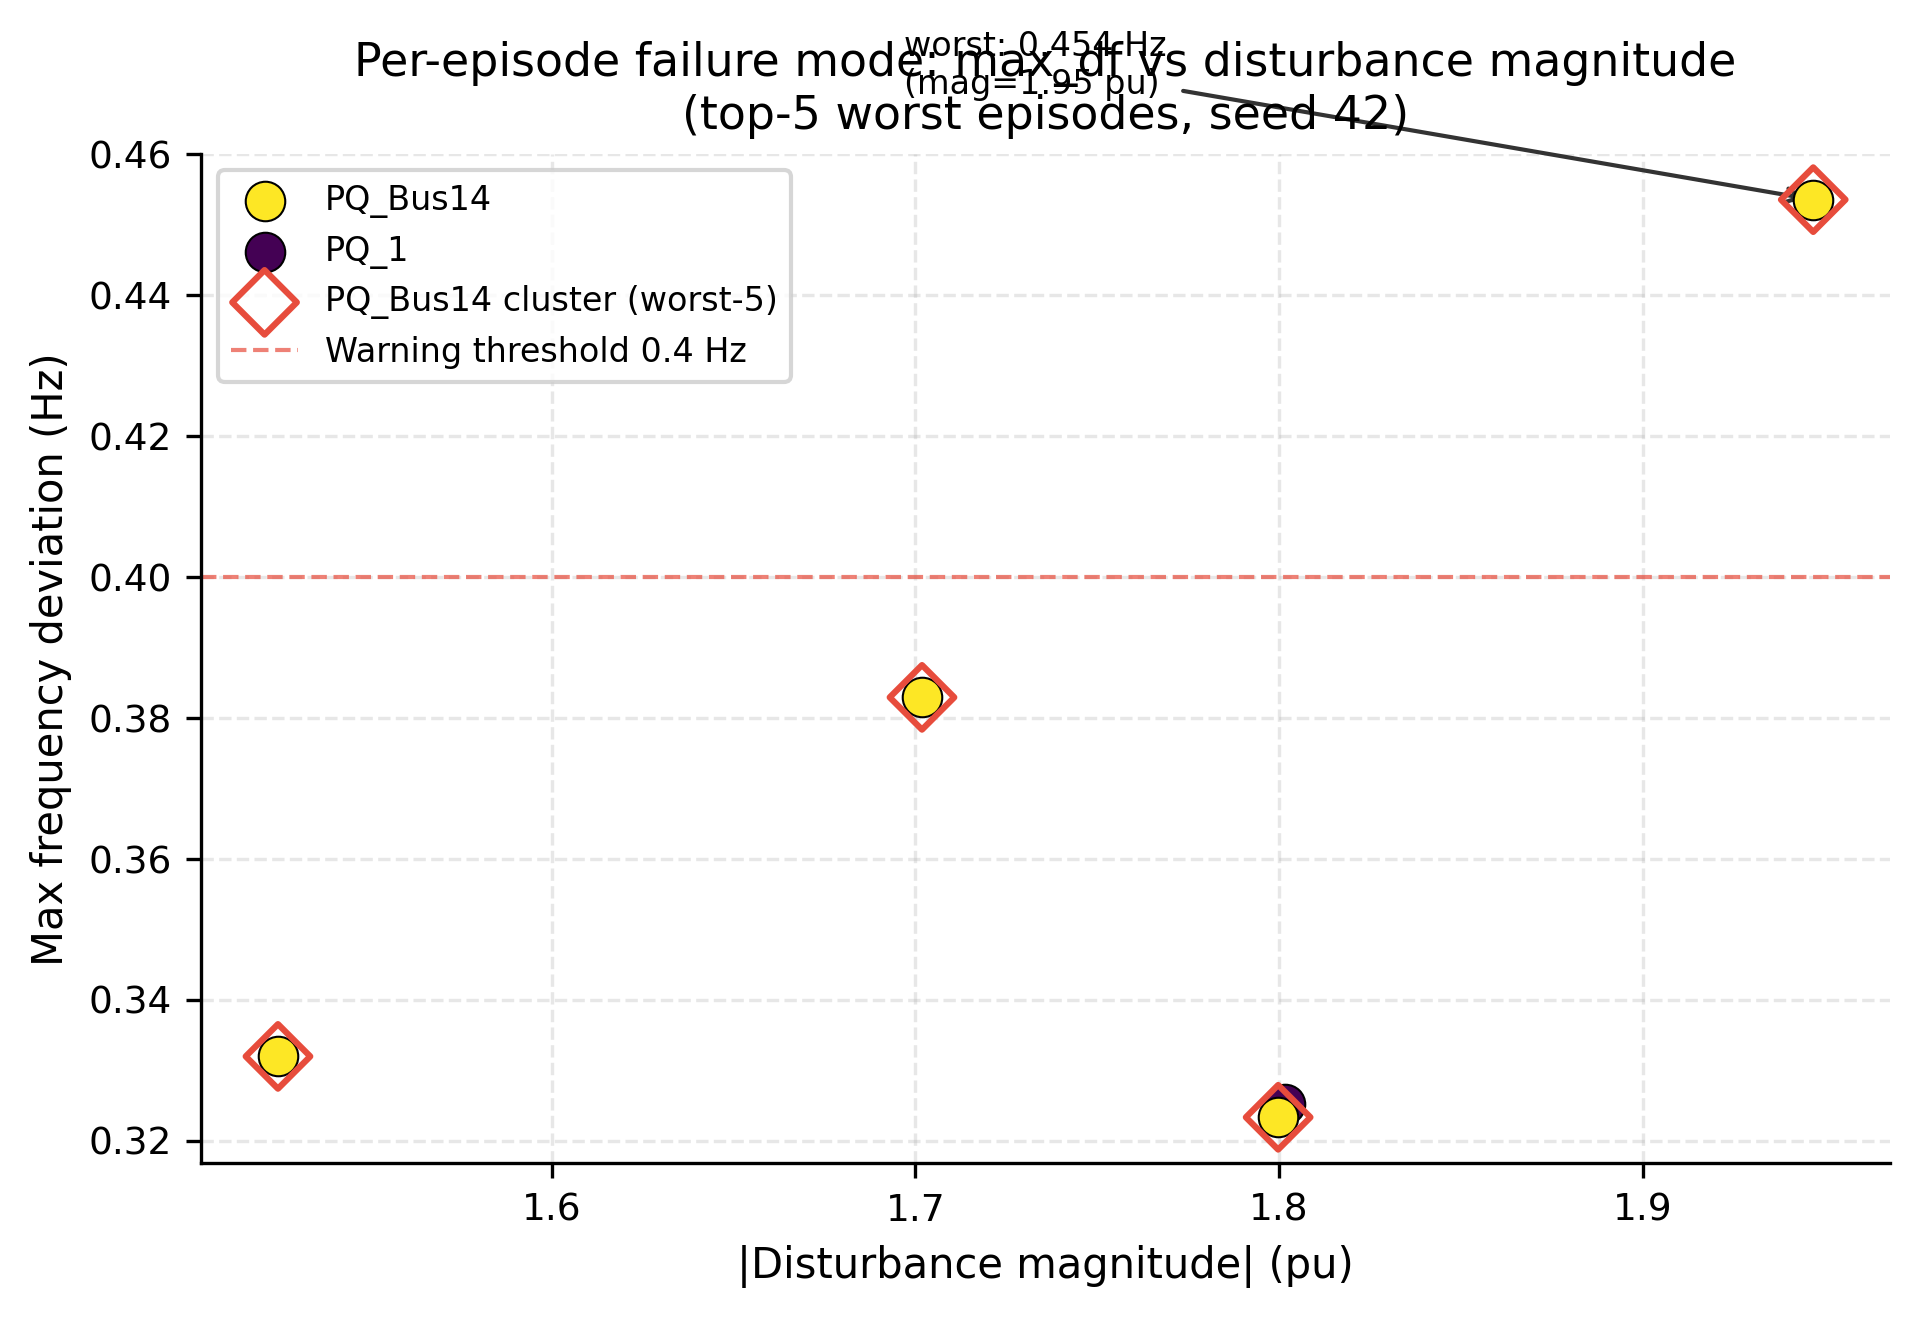
\includegraphics[width=0.92\columnwidth]{figures/fig5_worst_eps_scatter.png}
  \caption{Worst-five-episode scatter, max-$\Delta f$ vs.\ disturbance
  magnitude. PQ$_{\text{Bus14}}$ at $1.80$~p.u.\ dominates failure
  clusters across seeds (highlighted).}
  \label{fig:worst}
\end{figure}

\subsection{Triangulation: framework decoration}

Three independent observations converge on the same conclusion:
(i)~per-agent ablation shows $64\,\%$ mean dominance by one agent;
(ii)~shared-parameter SAC at $1/5$ training budget matches DDIC
(\cref{tab:phase9}); (iii)~shared-policy warmstart preserves the mean
within $\pm 8\,\%$ but does not improve it (\cref{tab:phase10}). On the
ANDES Kundur four-VSG system, the four-agent architecture contributes
no statistically measurable advantage over a one-agent shared policy.

\section{Honest Claims}\label{sec:claims}

\begin{enumerate}
  \item DDIC beats the uncontrolled baseline decisively: $3.36\times$
        on cum-$r_f$ at $n = 5$ seeds.
  \item DDIC ties tuned adaptive on cum-$r_f$ at $n = 5$: bootstrap
        and t-confidence intervals contain the adaptive mean. The
        $12\,\%$ point-estimate gap is not statistically significant.
  \item DDIC loses to adaptive on max-$\Delta f$ by $9$--$11\,\%$
        across both 3-seed and 5-seed cohorts.
  \item The DDIC/adaptive ratio reversed from the reference paper
        ($1.12$ ours vs.\ $0.62$ theirs) suggests the learning
        advantage does not transfer to a phasor-equilibrium backend.
  \item The multi-agent framework is decorative on this system. Three
        independent lines of evidence (\cref{sec:rootcause}) converge.
        A single shared-parameter policy at matched budget achieves
        equivalent performance.
  \item Failure modes are structural and bus-specific
        (PQ$_{\text{Bus14}}$ at $1.80$~p.u.).
  \item Project deviations are documented but material: hyperparameter
        rebalancing, action-range narrowing ($20\times$), and the
        ANDES backend collectively shift the optimization landscape.
        Absolute numbers are not directly comparable to the reference;
        qualitative ranking on paper-specific scenarios is preserved.
  \item Phase~10 warmstart pilot is filed as a null result:
        same-init does not break the structural dominance.
\end{enumerate}

\section{Limitations}\label{sec:limits}

\begin{itemize}
  \item \emph{Statistical sample}: $n = 5$ seeds with sample
        $\sigma = 0.265$ ($22\,\%$ of mean) triggers Gate A3
        (dispersion threshold). A non-overlapping-CI claim against
        adaptive would require Tier-B ($n = 10$) retraining.
  \item \emph{Adaptive baseline}: a generic
        proportional-derivative adaptive law $(K_H |\dot\omega|,\,
        K_D|\Delta\omega|)$ with a $5{\times}5$ K-grid sweep was
        chosen heuristically; tighter tuning may exist.
  \item \emph{Convergence at 500 episodes}: checkpoint-trajectory
        analysis on seed~42 shows agent~a1's share locks at $56.6\,\%$
        by episode~100 and remains within $1$~percentage point through
        episode~500. Longer training is unlikely to redistribute. We
        did not test $\geq 1000$ episodes.
  \item \emph{Cross-backend dominance}: an action-cosine probe
        suggests agents trained on Simulink show different
        differentiation than ANDES (Simulink: cos $\in [-0.08,\,+0.15]$;
        ANDES: $[+0.31,\,+0.35]$), but the definitive ablation test
        on Simulink requires a live MATLAB engine and is not run here.
  \item \emph{Other architectures untested}: centralized-training-
        decentralized-execution (CTDE) with a shared critic was not
        attempted; it is conceptually orthogonal to our findings and
        is a natural follow-up.
\end{itemize}

\section{Conclusion}\label{sec:conclusion}

We report an honest reproduction of multi-agent SAC for VSG
inertia/damping control on the ANDES Kundur four-bus system. DDIC
achieves a meaningful improvement over uncontrolled operation
($3.36\times$ on cum-$r_f$ at $n = 5$) but is not statistically better
than a tuned proportional-derivative adaptive baseline. Three
converging lines of evidence -- per-agent ablation showing $64\,\%$
mean dominance, a shared-parameter SAC matching DDIC at $1/5$ budget,
and a warmstart pilot that redistributes dominance without improving
the mean -- support the conclusion that the multi-agent framework is
decorative on this system.

We additionally identify three same-class evaluation bugs in which
evaluation scripts ran at $p_{\text{cf}} = 0$ while training used
$p_{\text{cf}} = 0.1$, inflating cum-$r_f$ by approximately $6\,\%$.
The corrected, paper-faithful evaluator and all training/eval
artifacts are released alongside this paper.

The reversal of the DDIC/adaptive performance ratio between Simulink
($0.62$, paper) and ANDES ($1.12$, this work) is consistent with
backend linearity: phasor-equilibrium dynamics are smoother and more
amenable to simple feedback control, leaving less room for SAC's
nonlinear value function. Future work should examine whether the
multi-agent advantage emerges only when EMT-grade nonlinear dynamics
are present, or whether the advantage in the original paper was an
artifact of evaluator construction or hyperparameter choices not
documented in the original work.

\section*{Reproducibility}

All training scripts, evaluators, audit reports, and the predraft
narrative are released. Key artifacts:

\begin{itemize}
  \item Training scripts:
        \texttt{scenarios/kundur/train\_andes.py},
        \texttt{train\_andes\_warmstart.py},
        \texttt{\_phase9\_shared\_param\_sac\_full.py}.
  \item Paper-grade evaluator:
        \texttt{scenarios/kundur/\_eval\_paper\_grade\_andes\_one.py}
        (single-controller worker) and \texttt{\_parallel.py}
        (5-process orchestrator).
  \item Agent-state probe (per-agent specialization, ablation, failure
        forensics): \texttt{probes/kundur/agent\_state/}.
  \item Audit reports: \texttt{quality\_reports/audits/2026-05-04\_*.md}
        (eval-discrepancy verdict, Tier-A $n = 5$ verdict, warmstart
        verdict, alpha-trajectory probe, agent-state cross-condition
        check).
  \item Predraft (this paper's primary source):
        \texttt{quality\_reports/replications/2026-05-03\_andes\_ddic\_honest\_results\_predraft.md}.
\end{itemize}

\bibliographystyle{IEEEtran}
\bibliography{refs}

\end{document}
